\chapter{Szimulációs eredmények}

\section{Szimulációs környezet}

A szimulációkat Python környezetben végeztem el, ahol a számítások jelentős részét a numpy könyvtár segítségével implementáltam, az eredmények értékeléséhez pedig a matplotlib könyvtárat használtam fel.
A szimuláció során egy Cella ID-ra vonatkoztatva végeztem el a méréseket, méghozzá a 120-as sorszámúra.
256 alvivővel végeztem a szimulációkat, így az $N_{FFT} = 256$.

A szimulált szinkronizációs jeleket a szabvány szerint generáltam, az egyetlen különbség az volt, hogy közöttük nem hagytam védőidőt, a PSS-t azonnal az SSS követi.
A két jel előtt és után védőidőt hagytam, itt csak zaj van a jelben.

\begin{figure}[h]
    \centering
    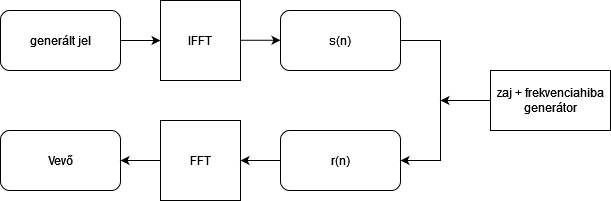
\includegraphics[keepaspectratio, width = 0.8\textwidth]{onlab.drawio.png}
    \caption{A szimulált rendszer blokkvázlata}
\end{figure}

A jelfeldolgozási és szinkronizációs feladatokat a vevő végzi el.
A szimulációt -45 dB és 5 dB között változó jel-zaj viszonnyal végeztem el, és mindegyik esetben 1000-szer szimuláltam egy szinkronizációs burstöt.

\section{PSS megkeresése}

\section{SSS dekódolása}

\section{Hibabecslés}



